% COMP1818 coursework report: EfficientNetV2-S progressive learning on low-data CIFAR-10.
% Structure follows the module's sample report (ECAI-style two-column paper):
%   Abstract, 1 Introduction, 2 Related Work, 3 Experiment and Results (3.1 Setup: 3.1.1 Dataset,
%   3.1.2 Model Design and Training, 3.1.3 Evaluation; 3.2 Results), 4 Discussion,
%   5 Conclusion and future work, 6 AI Use Reflection, References.
% If the module provides the official ECAI template (ecai.cls), paste the body into it instead.
% Compile: pdflatex main && pdflatex main   (references are inline; no BibTeX run needed)
% Every number comes from ../outputs (check with: python report/make_report_numbers.py).
\documentclass[10pt,twocolumn]{article}

\usepackage[a4paper,margin=0.7in,columnsep=0.25in]{geometry}
\usepackage[T1]{fontenc}
\usepackage[utf8]{inputenc}
\usepackage{times}
\usepackage{microtype}
\usepackage{amsmath,amssymb}
\usepackage{booktabs}
\usepackage{graphicx}
\usepackage{xcolor}
\usepackage{cite}
\usepackage[colorlinks=true,linkcolor=blue!60!black,citecolor=blue!60!black,urlcolor=blue!60!black]{hyperref}
\usepackage[font=small,labelsep=period,skip=3pt]{caption}
\usepackage{enumitem}
\setlist{nosep,leftmargin=*}
\usepackage{titlesec}
\titleformat{\section}{\normalfont\bfseries\large}{\thesection}{0.6em}{}
\titleformat{\subsection}{\normalfont\bfseries}{\thesubsection}{0.6em}{}
\titleformat{\subsubsection}{\normalfont\itshape}{\thesubsubsection}{0.6em}{}
\titlespacing*{\section}{0pt}{8pt plus 2pt}{4pt}
\titlespacing*{\subsection}{0pt}{6pt plus 2pt}{3pt}
\titlespacing*{\subsubsection}{0pt}{5pt plus 2pt}{2pt}

\setlength{\textfloatsep}{8pt plus 2pt minus 2pt}
\setlength{\floatsep}{6pt plus 2pt minus 2pt}
\setlength{\dbltextfloatsep}{8pt plus 2pt minus 2pt}

\newcommand{\pp}{\,pp}
\newcommand{\sx}{$\times$}
\newcommand{\todo}[1]{\textcolor{red}{#1}}

\title{\vspace{-1.2em}\textbf{Does Progressive Learning Transfer? EfficientNetV2-S\\ Fine-Tuning on Low-Data CIFAR-10}\vspace{-0.4em}}
\author{\todo{[Your full name]}\thanks{School of Computing and Mathematical Sciences,
University of Greenwich, London SE10 9LS, UK, email: \todo{[your university email]}}}
\date{\vspace{-1.8em}}

\begin{document}
\maketitle

\begin{abstract}
\noindent This study investigates whether the progressive learning of
EfficientNetV2~\cite{tan2021efficientnetv2}, which trains on small images with weak regularisation
before moving to larger images with stronger regularisation, still saves training time without losing
accuracy when a pretrained model is fine-tuned on a small image dataset. Four EfficientNetV2-S variants
(fixed 224\,px, growing image size only, the paper's full method, and the full method with Mixup) and
three baselines were trained for 12 epochs on the same 5{,}000 CIFAR-10 training images and 1{,}000
validation images, using a 4\,GB laptop GPU. On a separate test set of 2{,}000 images, the
fixed-resolution model achieved 95.35\% accuracy and a macro F1 score of 0.953, while the progressive
model achieved 95.50\% and 0.955 and needed 29\% less training time (1.40\sx, below the 1.56\sx\
predicted from FLOPs). Both were significantly more accurate than ResNet-18 (91.85\%) and far exceeded
HOG features with an SVM (54.10\%). However, the differences among the four EfficientNetV2-S variants
were not statistically significant, and only one random seed was used, so progressive learning cannot
be said to improve accuracy.
\end{abstract}

%=====================================================================
\section{Introduction}
%=====================================================================
Image classification assigns a category label to a photograph. Modern systems rarely learn this
from scratch: they fine-tune a network pretrained on ImageNet, often on a small dataset and modest
hardware. Two questions then decide which technique to use: how accurately it classifies, and how much
it costs to train.

EfficientNetV2~\cite{tan2021efficientnetv2} addresses both. Besides a fast-training architecture, it
introduces \emph{progressive learning}: images start small and grow during training, and
regularisation grows with them. The paper demonstrates this mainly for ImageNet-scale training; its
CIFAR-10 transfer experiments use the full training set and long schedules. Whether the method still
helps with a few thousand images, a short schedule and a laptop GPU is unclear.

This study classifies CIFAR-10~\cite{krizhevsky2009learning} images with 500 training images per class.
It compares hand-crafted features (HOG\,+\,SVM), a standard CNN (ResNet-18) and four training variants
of EfficientNetV2-S under the same splits, preprocessing and optimiser, and asks:
\textbf{RQ1}: How much more accurate are pretrained deep networks than hand-crafted features, and
EfficientNetV2-S than ResNet-18?
\textbf{RQ2}: Is progressive learning as accurate as fixed-resolution fine-tuning, and which part of
it (growing the size, adapting regularisation, or our Mixup extension) matters?
\textbf{RQ3}: Does its FLOPs saving become a wall-clock saving on a laptop GPU?

%=====================================================================
\section{Related Work}
%=====================================================================
EfficientNetV2 extends a line of efficient CNNs. MobileNetV2~\cite{sandler2018mobilenetv2} introduced
the inverted-residual block (MBConv), built around a depthwise $3{\times}3$ convolution;
Squeeze-and-Excitation~\cite{hu2018squeeze} added channel attention; MnasNet and
MobileNetV3~\cite{tan2019mnasnet,howard2019searching} searched over such blocks for fast inference; and
EfficientNet~\cite{tan2019efficientnet} scaled a searched network uniformly in depth, width and
resolution.

Tan and Le~\cite{tan2021efficientnetv2} found that this family trains slowly: large images use much
memory, depthwise convolutions run poorly on accelerators in early high-resolution layers, and uniform
scaling is sub-optimal. EfficientNetV2 therefore uses \emph{Fused-MBConv}~\cite{gupta2020accelerator},
which replaces the expansion and depthwise convolutions with one regular $3{\times}3$ convolution, in
early stages only (stages~1--3 of V2-S), and chooses its design with a search that rewards accuracy,
training speed and small size. Its \emph{progressive learning} splits training into $M$ stages; stage
$i$ uses image size $S_i$ and regularisation strengths $\phi_i^{k}$ (dropout,
RandAugment~\cite{cubuk2020randaugment} magnitude, Mixup~\cite{zhang2018mixup} $\alpha$), linearly
interpolated from start to end values:
\begin{equation}
S_i = S_0 + (S_e - S_0)\tfrac{i}{M-1},\qquad
\phi_i^{k} = \phi_0^{k} + (\phi_e^{k}-\phi_0^{k})\tfrac{i}{M-1}.
\label{eq:prog}
\end{equation}
Small images carry less information and so need weaker regularisation; the authors report that
resizing without adapting regularisation lost accuracy. For V2-S they use 128$\to$300\,px, RandAugment
5$\to$15, dropout 0.1$\to$0.3 and no Mixup, which they reserve for larger models.

Touvron et al.~\cite{touvron2019fixing} show that training and testing at different resolutions lowers
accuracy, which is why progressive training ends at its largest size. These studies use ImageNet-scale
data and budgets, so their accuracies are context rather than numbers to compare with ours.

%=====================================================================
\section{Experiment and Results}
%=====================================================================
\subsection{Setup}
\textbf{Implementation link:} \todo{[paste OneDrive/Google Drive/GitHub link to code, trained models and logs]}

\subsubsection{Dataset}
CIFAR-10~\cite{krizhevsky2009learning} contains 60{,}000 colour images of $32{\times}32$ pixels in ten
classes. With seed 42 we drew stratified, non-overlapping subsets: 500 images per class for training
and 100 per class for validation from the official training set, and 200 per class (2{,}000 images)
for testing from the official test set. Indices are saved in \texttt{outputs/splits.json}. Images were
upsampled to the training resolution and normalised with ImageNet statistics; every deep model used
random crops (4\,px padding) and horizontal flips.\\
\textbf{Dataset link:} \url{https://www.cs.toronto.edu/~kriz/cifar.html}

\subsubsection{Model Design and Training}
All deep models were ImageNet-pretrained torchvision~\cite{torchvision2016} checkpoints with a new
10-class head: EfficientNetV2-S (20.19\,M parameters) and ResNet-18~\cite{he2016deep} (11.18\,M). Each
was trained for 12 epochs with AdamW~\cite{loshchilov2019decoupled} (weight decay 0.05), one warm-up
epoch then cosine decay, batch size 32, label smoothing 0.1~\cite{szegedy2016rethinking} and mixed
precision. The learning rate $10^{-4}$ was chosen from $\{10^{-4}, 3{\times}10^{-4}, 10^{-3}\}$ by
validation accuracy in 3-epoch runs of variant A and used for every model. The four EfficientNetV2-S
variants were:
\begin{itemize}
\item \textbf{A} (fixed): 224\,px throughout, dropout 0.2, no RandAugment. ResNet-18 used the same settings.
\item \textbf{B0} (size only, our first extension): B's image sizes with A's regularisation, to separate
the effect of resizing (B0 vs A) from adapting regularisation (B vs B0).
\item \textbf{B} (paper recipe): size, RandAugment and dropout grow together over four 3-epoch stages
following Eq.~\eqref{eq:prog}, capped at 224\,px for the 4\,GB GPU (Table~\ref{tab:sched}).
\item \textbf{C} (Mixup ramp, our second extension): B plus Mixup, to test whether it helps V2-S when
only 5{,}000 images are available.
\end{itemize}

\begin{table}[t]
\centering\footnotesize
\begin{tabular}{@{}lcccc@{}}
\toprule
Stage (epochs) & 1 (1--3) & 2 (4--6) & 3 (7--9) & 4 (10--12) \\
\midrule
Image size (px) & 128 & 160 & 192 & 224 \\
RandAugment magnitude & 5 & 8 & 12 & 15 \\
Head dropout & 0.10 & 0.17 & 0.23 & 0.30 \\
Mixup $\alpha$ (C only) & 0 & 0.05 & 0.10 & 0.20 \\
\bottomrule
\end{tabular}
\caption{Progressive schedule for B and C. B0 uses only the size row.}
\label{tab:sched}
\end{table}

\subsubsection{Evaluation}
For each deep model, the epoch with the highest validation accuracy (always measured at 224\,px) was
selected and evaluated once on the 2{,}000 test images, which were used for no other choice. Accuracy is
the share of correctly classified images; macro-F1 averages the per-class F1 scores with equal weight.
McNemar's test~\cite{mcnemar1947note} checks whether two models differ, using the images that only one
of them classifies correctly. Baselines were uniform random guessing, always predicting the first
class, and HOG features~\cite{dalal2005histograms} with an RBF-kernel SVM ($C\in\{1,10\}$ chosen on
validation). Training cost is the wall-clock time of training steps only, on an NVIDIA RTX 2050 laptop
GPU (4\,GB) with PyTorch 2.14.1.

\subsection{Results}
\begin{table*}[t]
\centering\small
\resizebox{\textwidth}{!}{%
\begin{tabular}{@{}lcccccccc@{}}
\toprule
Model & Train res. (px) & Params (M) & Val acc. (\%) & Test acc. (\%) & Macro-F1 & Time (min) & Train--val gap (pp) & $p$ vs A \\
\midrule
Uniform random            & --          & --    & --    & 10.30 & 0.103 & --    & --  & -- \\
Majority class            & --          & --    & --    & 10.00 & 0.018 & --    & --  & -- \\
HOG + RBF-SVM ($C{=}1$)   & 32 (grey)   & --    & 54.30 & 54.10 & 0.541 & 0.1   & --  & $<10^{-100}$ \\
ResNet-18                 & 224         & 11.18 & 92.90 & 91.85 & 0.918 & 5.1   & 6.9 & $1.8{\times}10^{-8}$ \\
\midrule
A: EffNetV2-S, fixed      & 224         & 20.19 & 96.50 & 95.35 & 0.953 & 18.1  & 2.7 & -- \\
B0: progressive size only & 128$\to$224 & 20.19 & 96.10 & 95.05 & 0.951 & 12.4  & 3.1 & 0.58 \\
B: progressive (paper)    & 128$\to$224 & 20.19 & 96.70 & 95.50 & 0.955 & 12.9  & 0.1 & 0.81 \\
C: B + Mixup ramp         & 128$\to$224 & 20.19 & 96.10 & 95.35 & 0.953 & 13.0  & n/a$^\dagger$ & 0.91 \\
\bottomrule
\end{tabular}}
\caption{Test results on 2{,}000 CIFAR-10 images (one run per model, seed 42). Validation accuracy is at
the selected epoch; time is training-step wall-clock time; the train--val gap is measured at the
selected epoch on augmented training inputs. $p$ is McNemar's test against A. $^\dagger$Not comparable
under Mixup, where training accuracy uses mixed labels.}
\label{tab:main}
\end{table*}

\paragraph{Accuracy (RQ1, RQ2).} Table~\ref{tab:main} shows that both trivial baselines sit at chance,
confirming balanced splits. Pretrained deep networks far outperformed hand-crafted features: HOG + SVM
reached 54.10\%, every deep model over 91\%. With the same recipe, EfficientNetV2-S (A) was 3.5\pp\ more
accurate than ResNet-18 (95.35 vs 91.85\%, $p=1.8{\times}10^{-8}$), at 3.5\sx\ the training time; all four
variants beat ResNet-18 significantly ($p\leq3.2{\times}10^{-7}$). Among the variants, B scored highest
(95.50\%, macro-F1 0.955), but \emph{no pair among A, B0, B and C differed significantly} (all
$p>0.3$). The 95\% confidence interval on one accuracy is about $\pm0.9$\pp, larger than the 0.45\pp\
spread between the variants.

\begin{figure}[t]
\centering
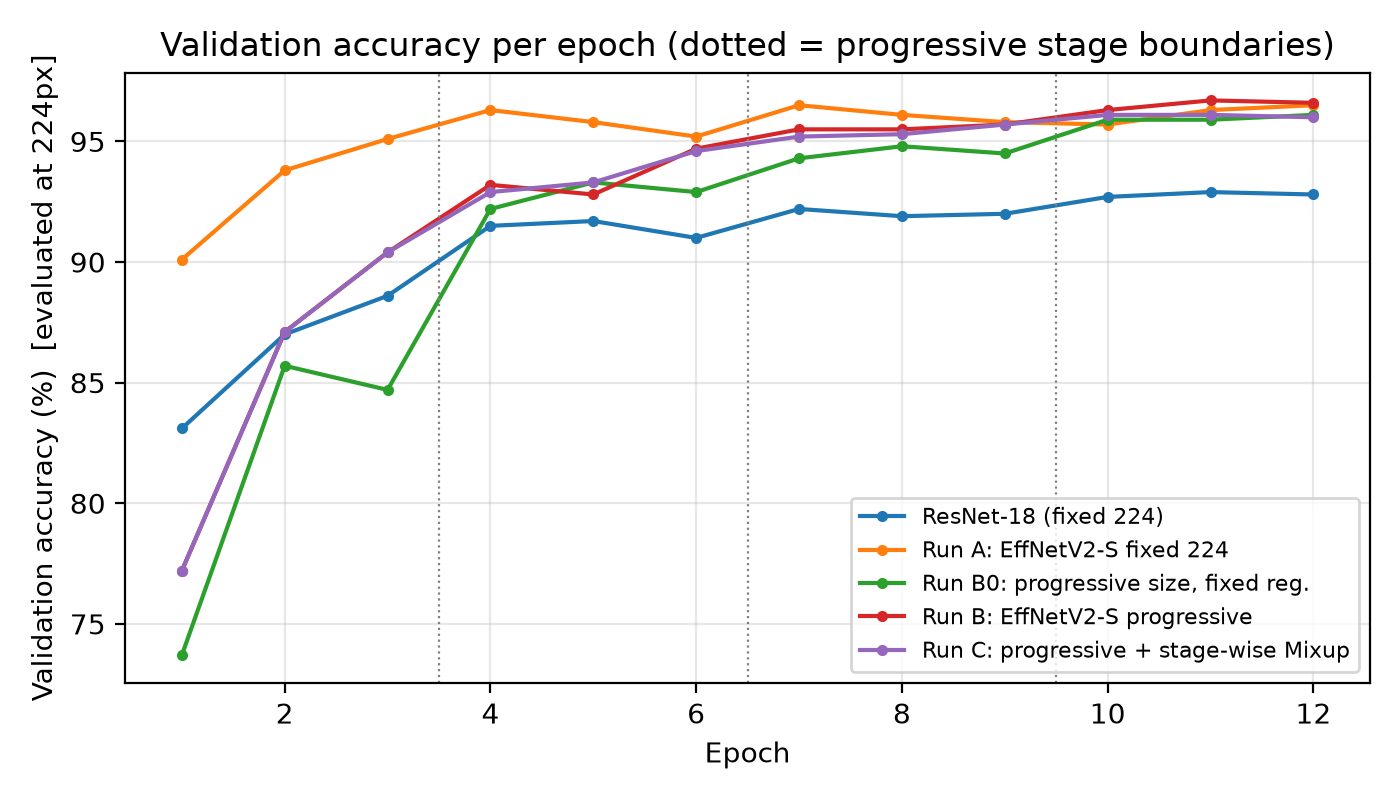
\includegraphics[width=\columnwidth]{figures/val_acc_comparison.png}
\caption{Validation accuracy (at 224\,px) per epoch. Dotted lines mark the stage boundaries of B0, B
and C.}
\label{fig:val}
\end{figure}

\paragraph{Learning curves.} In Figure~\ref{fig:val}, the progressive variants started 13--16\pp\ below
A because they trained at 128\,px but were validated at 224\,px~\cite{touvron2019fixing}; the gap had
closed by stage~4, when the resolutions matched. A and B0 reached about 99\% training accuracy (a
2.7--3.1\pp\ gap to validation), whereas B ended with a 0.1\pp\ gap at equal or higher validation
accuracy.

\paragraph{Class-level performance.} Figure~\ref{fig:cm} shows predictions per class. Frog had the
highest recall under both A and B (197 of 200) and cat the lowest (174 and 179). For A, B and ResNet-18
the most common confusion was between cat and dog (a cat predicted as a dog 17 times under A, 13 under
B), followed by automobile and truck. B classified more cats, birds, automobiles and horses correctly
than A, but fewer trucks (189 vs 194), ships (193 vs 196) and dogs (185 vs 187), so its small lead is
not consistent across classes.

\begin{figure*}[t]
\centering
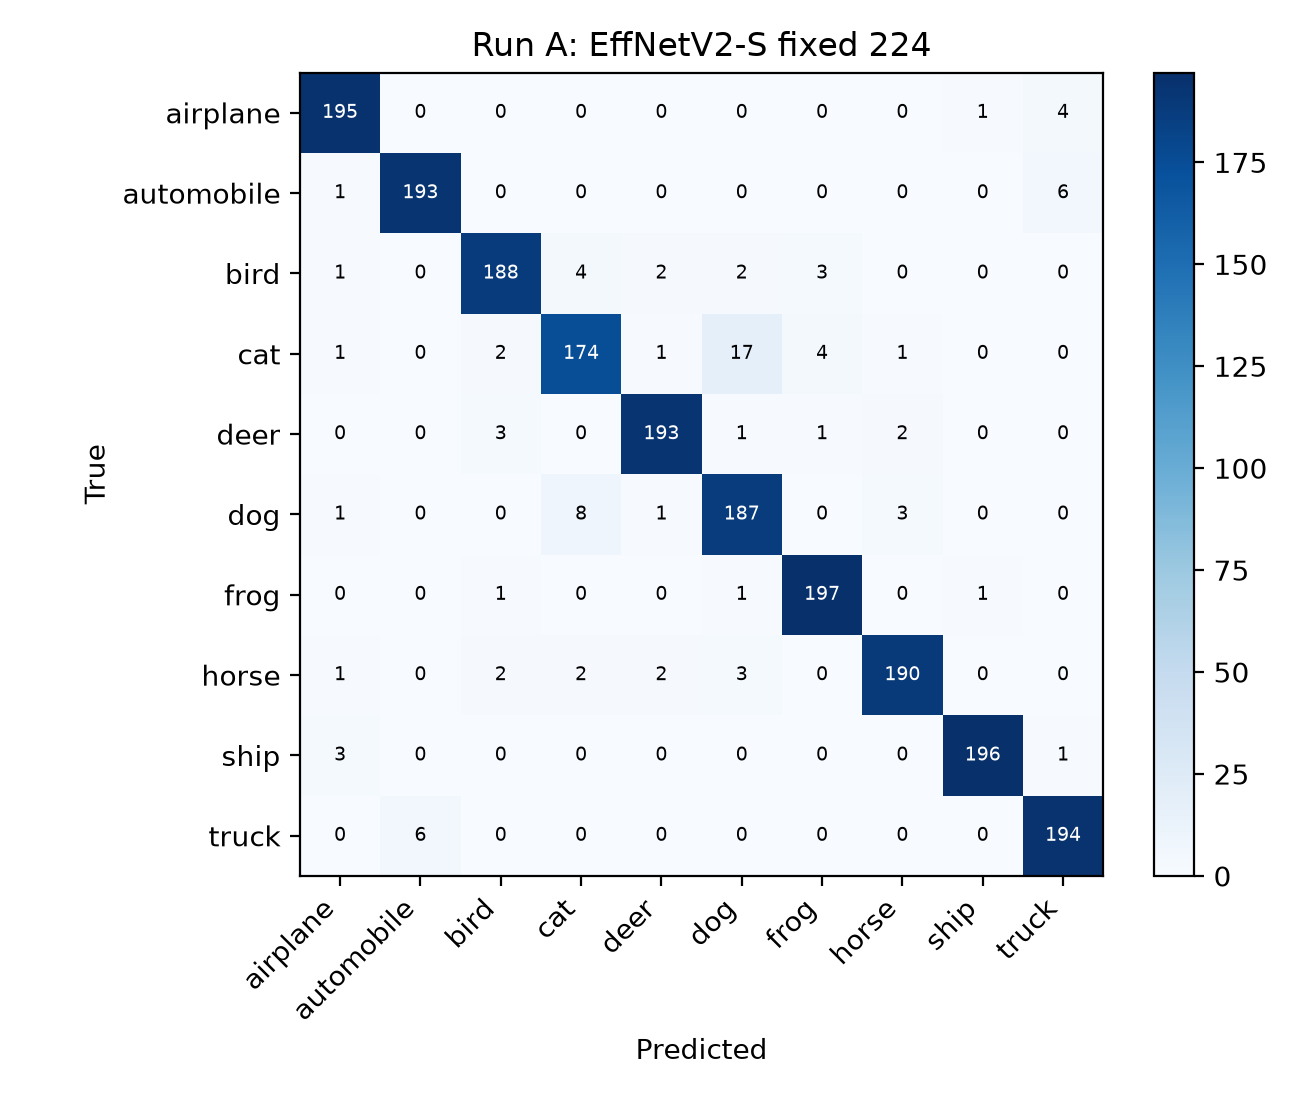
\includegraphics[width=0.36\textwidth]{figures/cm_A_effnetv2s_fixed224.png}\hspace{2em}
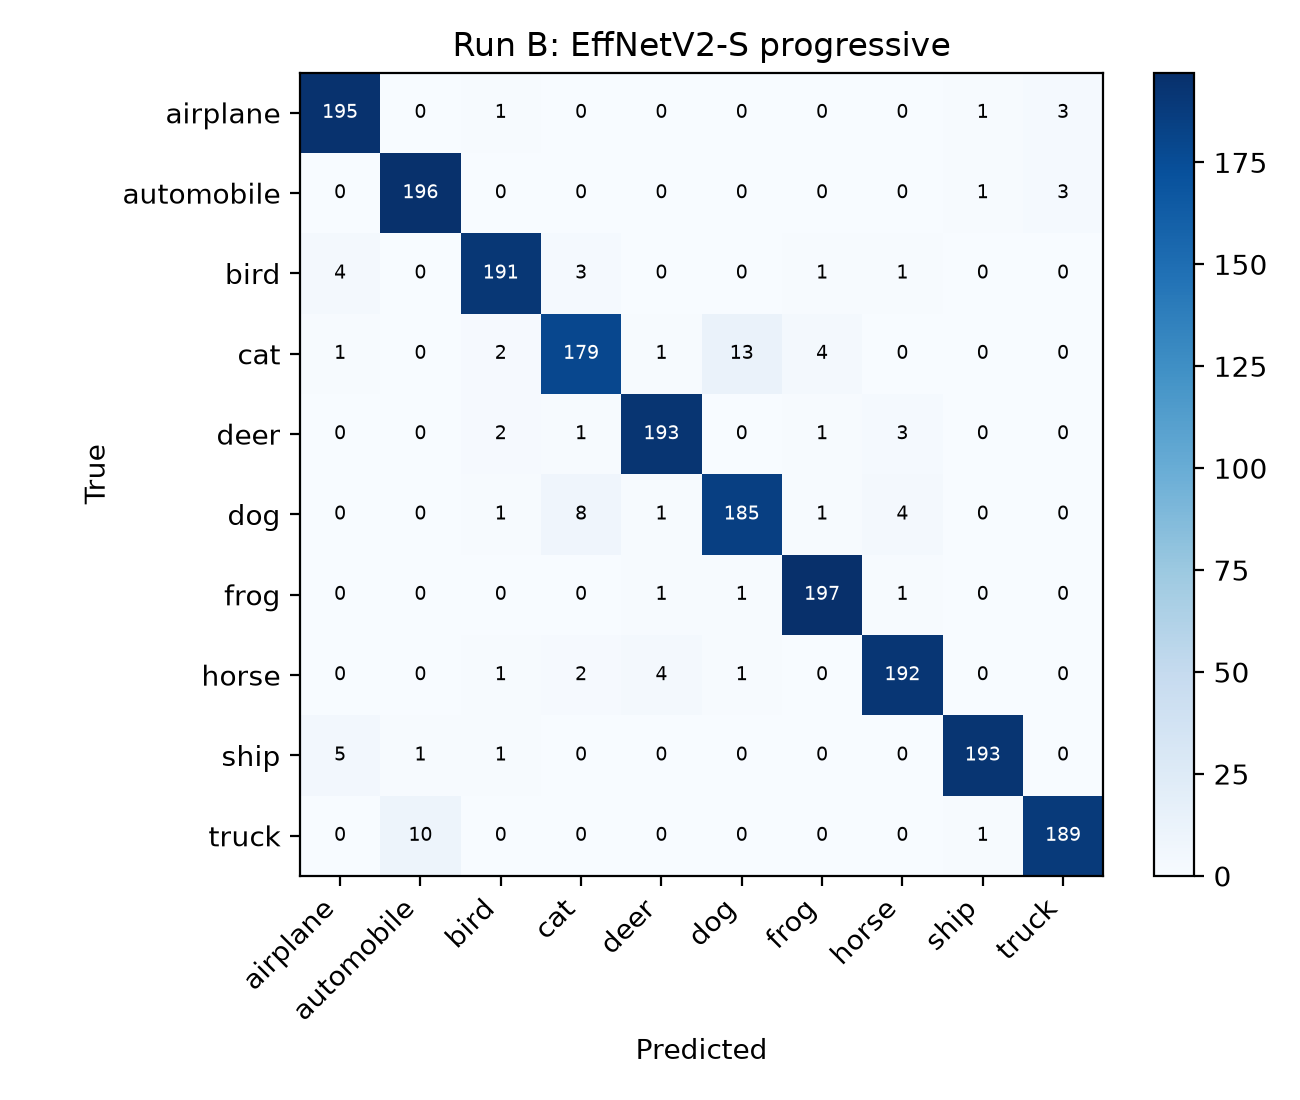
\includegraphics[width=0.36\textwidth]{figures/cm_B_effnetv2s_progressive.png}
\caption{Test confusion matrices for A (left) and B (right). Rows are true labels; columns are
predictions; each class has 200 test images.}
\label{fig:cm}
\end{figure*}

\paragraph{Training cost (RQ3).} Training time fell from 18.1\,min (A) to 12.9\,min (B, 1.40\sx), 12.4\,min
(B0, 1.45\sx) and 13.0\,min (C, 1.39\sx). FLOPs grow with $(S/224)^2$, predicting 0.643 of A's cost
(1.56\sx). A least-squares fit over all 48 EfficientNetV2-S epochs gives
\begin{equation}
t_{\text{epoch}}(S) \approx 15.7\,\text{s} + 74.8\,\text{s}\cdot(S/224)^2,\qquad R^2=0.991,
\label{eq:cost}
\end{equation}
which predicts a ratio of 0.705, within 0.02 of each measured value: about 17\% of a 224\,px epoch is a
fixed cost that does not shrink with image size. Peak GPU memory was unchanged (2.62--2.63\,GB), as it
is set by the final 224\,px stage.

%=====================================================================
\section{Discussion}
%=====================================================================
For classification accuracy (RQ1), pretraining matters most: the 38--41\pp\ gap between HOG + SVM and
the deep models dwarfs every other difference. Architecture comes next: EfficientNetV2-S was
significantly more accurate than ResNet-18 under an identical recipe, though it has more parameters and
trained 3.5\sx\ longer, so the gain cannot be attributed to its design alone.

For RQ2, there is no evidence that progressive learning costs accuracy, but the experiment cannot show
that the variants are equivalent: with one seed and 2{,}000 test images, differences below about 1\pp\
are not resolvable. Resizing alone (B0 vs A) changed accuracy by $-0.30$\pp\ ($p=0.58$), adaptive
regularisation (B vs B0) by $+0.45$\pp\ ($p=0.35$) while narrowing the train--validation gap, and the
Mixup ramp (C vs B) by $-0.15$\pp\ ($p=0.79$). None is significant. CIFAR-10 also limits this test:
every resolution is an interpolation of the same $32{\times}32$ image, so small stages lose no
information, which weakens the paper's argument that small images need less regularisation.

For RQ3, the cost model attributes the shortfall from 1.56\sx\ to a fixed cost per epoch. Likely
sources are the small GPU, the batch of 32 and single-process data loading, though these were not
profiled. FLOPs, as EfficientNetV2 itself argues, do not equal training time.

Other limitations: the learning rate was tuned on A and reused, which may slightly favour A; selecting
the best epoch on 1{,}000 validation images is mildly optimistic for every model; and the study caps
images at 224\,px and trains for 12 epochs instead of the paper's 300\,px and about 350 epochs, so it
tests the mechanism in transfer rather than the paper's reported numbers.

%=====================================================================
\section{Conclusion and future work}
%=====================================================================
This study compared techniques for classifying CIFAR-10 images with 500 training images per class.
Pretrained deep networks far outperformed HOG + SVM (54.10\%), and EfficientNetV2-S was significantly
more accurate than ResNet-18 (95.35 vs 91.85\%, $p=1.8{\times}10^{-8}$). Progressive learning was
statistically indistinguishable from fixed-resolution fine-tuning (95.50 vs 95.35\%, $p=0.81$) and cut
training time by 29\%, less than the 36\% implied by FLOPs because of a fixed per-epoch cost. Neither
adaptive regularisation nor Mixup changed accuracy significantly. Progressive learning therefore saved
training time at no detectable cost in accuracy under the tested conditions, but did not improve
accuracy. Future work could use several random seeds, natively high-resolution images where small
stages genuinely remove detail, and faster data loading to recover more of the FLOPs saving.

%=====================================================================
\section{AI Use Reflection}
%=====================================================================
% REQUIRED: 60-100 words, written by you. Cover: (1) which AI tool(s) you used; (2) how AI supported
% your learning; (3) how you edited, transformed or expanded the AI outputs; (4) how you verified the
% outputs and corrected errors (for example, checking numbers against outputs/*.json and the logs).
% Be specific and honest about what AI produced (code, figures, text) and what you did yourself.
\todo{[Write your 60--100 word reflection here.]}

% Optional, as in the sample report:
% \section*{Acknowledgements}
% ...

{\small
\begin{thebibliography}{99}
\setlength{\itemsep}{1pt}

\bibitem{cubuk2020randaugment}
Ekin~D. Cubuk, Barret Zoph, Jonathon Shlens, and Quoc~V. Le, `RandAugment: Practical automated data
augmentation with a reduced search space', in \emph{IEEE/CVF Conference on Computer Vision and Pattern
Recognition Workshops}, pp. 702--703, (2020).

\bibitem{dalal2005histograms}
Navneet Dalal and Bill Triggs, `Histograms of oriented gradients for human detection', in \emph{IEEE
Computer Society Conference on Computer Vision and Pattern Recognition}, volume~1, pp. 886--893, (2005).

\bibitem{gupta2020accelerator}
Suyog Gupta and Berkin Akin, `Accelerator-aware neural network design using AutoML', \emph{arXiv
preprint arXiv:2003.02838}, (2020).

\bibitem{he2016deep}
Kaiming He, Xiangyu Zhang, Shaoqing Ren, and Jian Sun, `Deep residual learning for image recognition',
in \emph{IEEE Conference on Computer Vision and Pattern Recognition}, pp. 770--778, (2016).

\bibitem{howard2019searching}
Andrew Howard, Mark Sandler, Grace Chu, Liang-Chieh Chen, Bo~Chen, Mingxing Tan, Weijun Wang, Yukun Zhu,
Ruoming Pang, Vijay Vasudevan, Quoc~V. Le, and Hartwig Adam, `Searching for MobileNetV3', in
\emph{IEEE/CVF International Conference on Computer Vision}, pp. 1314--1324, (2019).

\bibitem{hu2018squeeze}
Jie Hu, Li~Shen, and Gang Sun, `Squeeze-and-excitation networks', in \emph{IEEE Conference on Computer
Vision and Pattern Recognition}, pp. 7132--7141, (2018).

\bibitem{krizhevsky2009learning}
Alex Krizhevsky, `Learning multiple layers of features from tiny images', Technical report,
University of Toronto, (2009).

\bibitem{loshchilov2019decoupled}
Ilya Loshchilov and Frank Hutter, `Decoupled weight decay regularization', in \emph{International
Conference on Learning Representations}, (2019).

\bibitem{mcnemar1947note}
Quinn McNemar, `Note on the sampling error of the difference between correlated proportions or
percentages', \emph{Psychometrika}, \textbf{12}(2), 153--157, (1947).

\bibitem{sandler2018mobilenetv2}
Mark Sandler, Andrew Howard, Menglong Zhu, Andrey Zhmoginov, and Liang-Chieh Chen, `MobileNetV2:
Inverted residuals and linear bottlenecks', in \emph{IEEE Conference on Computer Vision and Pattern
Recognition}, pp. 4510--4520, (2018).

\bibitem{szegedy2016rethinking}
Christian Szegedy, Vincent Vanhoucke, Sergey Ioffe, Jon Shlens, and Zbigniew Wojna, `Rethinking the
Inception architecture for computer vision', in \emph{IEEE Conference on Computer Vision and Pattern
Recognition}, pp. 2818--2826, (2016).

\bibitem{tan2019mnasnet}
Mingxing Tan, Bo~Chen, Ruoming Pang, Vijay Vasudevan, Mark Sandler, Andrew Howard, and Quoc~V. Le,
`MnasNet: Platform-aware neural architecture search for mobile', in \emph{IEEE/CVF Conference on
Computer Vision and Pattern Recognition}, pp. 2820--2828, (2019).

\bibitem{tan2019efficientnet}
Mingxing Tan and Quoc~V. Le, `EfficientNet: Rethinking model scaling for convolutional neural
networks', in \emph{Proceedings of the 36th International Conference on Machine Learning}, PMLR~97,
pp. 6105--6114, (2019).

\bibitem{tan2021efficientnetv2}
Mingxing Tan and Quoc~V. Le, `EfficientNetV2: Smaller models and faster training', in
\emph{Proceedings of the 38th International Conference on Machine Learning}, PMLR~139,
pp. 10096--10106, (2021).

\bibitem{torchvision2016}
TorchVision maintainers and contributors, `TorchVision: PyTorch's computer vision library',
\url{https://github.com/pytorch/vision}, (2016). Pretrained EfficientNetV2-S and ResNet-18 weights.

\bibitem{touvron2019fixing}
Hugo Touvron, Andrea Vedaldi, Matthijs Douze, and Herv{\'e} J{\'e}gou, `Fixing the train-test
resolution discrepancy', in \emph{Advances in Neural Information Processing Systems}, volume~32, (2019).

\bibitem{zhang2018mixup}
Hongyi Zhang, Moustapha Cisse, Yann~N. Dauphin, and David Lopez-Paz, `mixup: Beyond empirical risk
minimization', in \emph{International Conference on Learning Representations}, (2018).

\end{thebibliography}
}

\end{document}
